\documentclass[11pt,a4paper]{article}
\usepackage[utf8]{inputenc}
\usepackage[T1]{fontenc}
\usepackage{amsmath}
\usepackage{amssymb}
\usepackage{amsfonts}
\usepackage{graphicx}
\usepackage{hyperref}
\usepackage{geometry}
\usepackage{authblk}
\usepackage{tikz}
\usetikzlibrary{positioning, arrows.meta, shapes.geometric}

\geometry{a4paper, margin=1in}

\title{Mastering Heads-Up No-Limit Texas Hold'em with Deep Counterfactual Regret Minimization and Transformer Architectures}

% Authorship can be customized as needed
\author[1]{AI Research Group}
\affil[1]{(Organization/Affiliation)}

\date{August 2025}

\begin{document}

\maketitle

\begin{abstract}
Heads-Up No-Limit Texas Hold'em (HU NLHE) presents a monumental challenge for Artificial Intelligence due to its imperfect-information nature and vast state space (on the order of $10^{75}$ game states for standard competitive variants). Traditional Counterfactual Regret Minimization (CFR) methods are computationally intractable at this scale. This paper presents a comprehensive framework for developing a state-of-the-art HU NLHE AI using Deep Counterfactual Regret Minimization (Deep CFR), which leverages deep neural networks for function approximation. We focus on a Transformer-based advantage network, arguing that self-attention is well suited to capturing long-range dependencies in betting sequences while respecting information constraints. We detail implementation strategies, including structured infoset representation with permutation-invariant card encoding, efficient training via Linear CFR (LCFR) with normalized weighted regression, robust handling of off-tree actions (action translation with optional subgame re-solving), and validation practices that prevent common CFR errors.
\end{abstract}

\section{Introduction}

The pursuit of solving imperfect-information games has been a driving force in AI research. No-Limit Texas Hold'em (NLHE), characterized by hidden information and a massive action space, serves as a primary benchmark. In this work we explicitly target \textbf{two-player zero-sum HU NLHE} to align with CFR's theoretical guarantees. Milestones such as Libratus \cite{brown2017superhuman} and Pluribus \cite{brown2019superhuman} demonstrated superhuman performance in large poker settings through abstraction and real-time solving; DeepStack \cite{moravcik2017deepstack} and ReBeL \cite{brown2020rebel} integrated learning with search. Our contribution is a practically grounded, end-to-end Deep CFR blueprint that replaces tabular regrets with a \emph{Transformer} advantage function and a modern training pipeline suitable for HU NLHE.

CFR \cite{zinkevich2007regret} is an iterative algorithm that converges to a Nash equilibrium in zero-sum games by minimizing regret. However, standard tabular CFR requires storing regrets for every information set, which is infeasible in full-scale NLHE.

Deep CFR \cite{brown2018deep} addresses this scalability issue by replacing tabular regrets with function approximation. These networks generalize strategic knowledge across similar information sets, mitigating the need for manual information abstraction. We also discuss a Single Deep CFR (SD-CFR) style reconstruction of the average strategy that avoids training a separate strategy network \cite{steinberger2019sdcfr}.

This paper advances Deep CFR by integrating Transformer architectures \cite{vaswani2017attention}. Poker is inherently sequential: the meaning of a river bet depends on pre-flop action and public-card reveals. Self-attention lets the model weigh distant events in the betting history. We further encode private/public \emph{card sets} with permutation-invariant attention (Set Transformer) \cite{lee2019settransformer} before fusing them with the bet-history encoder.

\section{Preliminaries and CFR Foundations}

\subsection{Game Theory Concepts}

We model NLHE as an extensive-form game.
\begin{itemize}
    \item \textbf{Histories (H):} A sequence of actions (by players or chance) starting from the initial state.
    \item \textbf{Information Set (Infoset, I):} A partition of the histories belonging to a player $i$, such that all histories in $I$ are indistinguishable to player $i$. In poker, $I$ is defined by the player's private cards, public cards, and the complete betting history.
    \item \textbf{Strategy Profile ($\sigma$):} A collection of strategies, where $\sigma_i(I)(a)$ is the probability that player $i$ takes action $a$ at infoset $I$.
\end{itemize}

\subsection{Counterfactual Regret Minimization (CFR)}

CFR iteratively updates strategies by minimizing regret. A crucial concept is the \textbf{Counterfactual Value (CFV)}. The CFV for player $i$ at infoset $I$ under strategy profile $\sigma$ is the expected utility, weighted by the probability that opponents and chance allow the state to be reached ($\pi_{-i,\text{chance}}^\sigma(I)$). This weighting is critical for focusing optimization on strategically reachable parts of the game tree.

The immediate regret (or advantage) for action $a$ at infoset $I$ in iteration $T$ is:
\begin{equation}
r^T(I, a) = v^\sigma(I, a) - v^\sigma(I)
\end{equation}
Where $v^\sigma(I, a)$ is the CFV of taking action $a$ and then following $\sigma$, and $v^\sigma(I)$ is the average CFV at $I$ under $\sigma$.

The cumulative regret is updated as:
\begin{equation}
R^T(I, a) = R^{T-1}(I, a) + r^T(I, a)
\end{equation}

\textbf{Regret Matching:} The strategy for the next iteration is determined by making actions proportional to their positive cumulative regret:
\begin{equation}
\sigma^{T+1}(I, a) = \frac{R_{+}^{T}(I, a)}{\sum_{a' \in A(I)} R_{+}^{T}(I, a')}
\end{equation}
If the denominator is zero, a uniform random strategy is used.

\section{Deep Counterfactual Regret Minimization (Deep CFR)}

Deep CFR approximates the behavior of CFR in large games by using neural networks to generalize across the vast space of infosets.

\subsection{Architecture Overview}

There are two established approaches:

\begin{enumerate}
    \item \textbf{Advantage (Regret) Network ($V_A$):} Parameterized by $\theta_A$, it approximates immediate advantages at a given infoset, $V_A(I;\theta_A)\approx r(I,\cdot)$.
    \item \textbf{Average strategy reconstruction:} (a) \emph{Deep CFR} trains a separate strategy network from a strategy-memory buffer using sample weights (LCFR) \cite{brown2018deep}. (b) \emph{SD-CFR} reconstructs the average strategy by sampling from the collection of advantage networks saved across iterations, avoiding a separate strategy network \cite{steinberger2019sdcfr}.
\end{enumerate}

In this paper we adopt \textbf{SD-CFR-style reconstruction} to avoid compounding approximation error. We checkpoint the advantage network $V_A$ periodically (e.g., every $N$ iterations). At inference time, to approximate the average strategy, we first uniformly sample a checkpointed network $V_A^k$ from the set of all saved checkpoints. Then, for the duration of a single game, we derive the policy at each infoset $I$ by applying regret matching to the advantages predicted by that specific network, $V_A^k(I; \theta_A^k)$. This avoids training a separate, and potentially lagging, strategy network. All function approximation is implemented with Transformers.

\subsection{Training Procedure: Sampling and Learning}

Deep CFR interleaves data generation (traversal) and network optimization.

\subsubsection{Game Traversal (Data Generation)}

Since the full game tree cannot be traversed, Deep CFR employs Monte Carlo CFR (MCCFR), most commonly \textbf{External Sampling}. External Sampling samples the actions of the opponent(s) and chance events, while iterating over all possible actions for the player being optimized (the "traverser"). This yields lower variance updates.

During traversal, the system queries $V_A$ to determine the current strategy $\sigma^T$, calculates the realized CFVs, computes the realized immediate regrets $r^T(I, a)$, and stores the tuple $(I, r^T(I, a), T)$ in the Advantage Memory Buffer ($M_A$).

\subsubsection{Network Training}

The Advantage Network $V_A$ is trained via supervised learning on the data in $M_A$. The objective is to minimize the difference between the network's predictions and the realized advantages.

\subsection{Stabilization and Optimization}

\begin{itemize}
    \item \textbf{Reservoir Sampling:} Memory buffers ($M_A$) use reservoir sampling to maintain a fixed-size buffer representing a uniform sample of all generated data, crucial for convergence properties.
    \item \textbf{Linear CFR (LCFR):} To accelerate convergence, samples are weighted by the iteration index $T$.
    \item \textbf{VR-MCCFR (optional):} Variance-reduction baselines can be added to further stabilize estimates without changing the training interface \cite{schmid2018vrmccfr}.
\end{itemize}

Crucially, LCFR weights must be incorporated into the loss function. We use a \emph{normalized} weighted MSE to keep gradient scales stable across batches with different iteration mixes:

\begin{equation}
L(\theta_A) = \frac{\sum_{(I, r, T) \in B} T \,\big\| V_A(I;\theta_A) - r \big\|^2}{\sum_{(I, r, T) \in B} T}
\end{equation}

Where $B$ is the training batch, $\theta_A$ are the network parameters, and $T$ is the iteration number when the sample was generated. Failure to implement this weighted loss correctly will severely hamper convergence.

\section{Applying Transformer Architectures to Poker}

The sequential nature of poker makes it highly suitable for the Transformer architecture. Self-attention allows the model to process the entire game sequence simultaneously and identify relevant relationships between distant events (e.g., relating a river bet back to pre-flop actions).

\subsection{Structured Game State Representation (Input Encoding)}

Encoding the poker infoset requires careful design. A structured approach separates static context from the dynamic history and treats cards as \emph{sets}.

\begin{enumerate}
    \item \textbf{Tokenization:} The game history is treated as a sequence of events.
    \begin{itemize}
        \item \textit{Action Tokens:} Represent the type of action (e.g., \texttt{[RAISE]}, \texttt{[CALL]}).
        \item \textit{Card Tokens:} Represent rank and suit (e.g., \texttt{[As]}).
    \end{itemize}

    \item \textbf{Card Set Encoder (Permutation-Invariant):} Hole cards and public cards (flop/turn/river) are sets. We encode each set with a small Set Transformer \cite{lee2019settransformer} and produce fixed-size summaries per street that do not depend on arbitrary card order.

    \item \textbf{Feature Augmentation and Normalization:} Action tokens are augmented with associated scalars (bet sizes, stack depths) normalized as fractions of pot or stacks (optionally log-scaled). Scalars are projected and fused with the token embeddings.

    \item \textbf{Structured Input Construction:} The input sequence $X$ is constructed by concatenating different segments:
    \begin{itemize}
        \item \textbf{Prefix (Static Context):} Encoded hole cards (set encoder), positions, stack-and-blind configuration.
        \item \textbf{Sequence (Dynamic History):} The sequential history of betting actions and the revelation of community cards (Flop, Turn, River).
    \end{itemize}

    \item \textbf{Positional and Round Encoding:} The order of events is crucial. Positional encodings (sinusoidal or learned) must be added. Furthermore, 'Round-aware' segment embeddings (Pre-flop, Flop, Turn, River) are often added to explicitly delineate the betting rounds.

    \item \textbf{Information Hiding:} The infoset representation must strictly only encode information visible to the acting player. Opponent hole cards must never be included in the input.

\end{enumerate}

\subsection{Network Architecture}

We adapt a Transformer Encoder for the advantage network ($V_A$). Because the entire history up to the decision point is available, causal masking is unnecessary. All modules in our system are Transformer-based; we do not use LSTMs.

\begin{itemize}
    \item \textbf{Card Set Encoders:} Set Transformer blocks summarize hole cards and public-card sets per street.
    \item \textbf{History Encoder:} A stack of Transformer encoder blocks processes the action/history sequence with positional and round embeddings.
    \item \textbf{Fusion and Head:} We concatenate card-set summaries with the pooled history representation (e.g., \texttt{[CLS]} or mean-pooled) and pass through a linear head to output advantages for the discretized legal actions. Illegal actions are masked prior to regret-matching.
\end{itemize}

% TikZ Diagram
\begin{figure}[h]
\centering
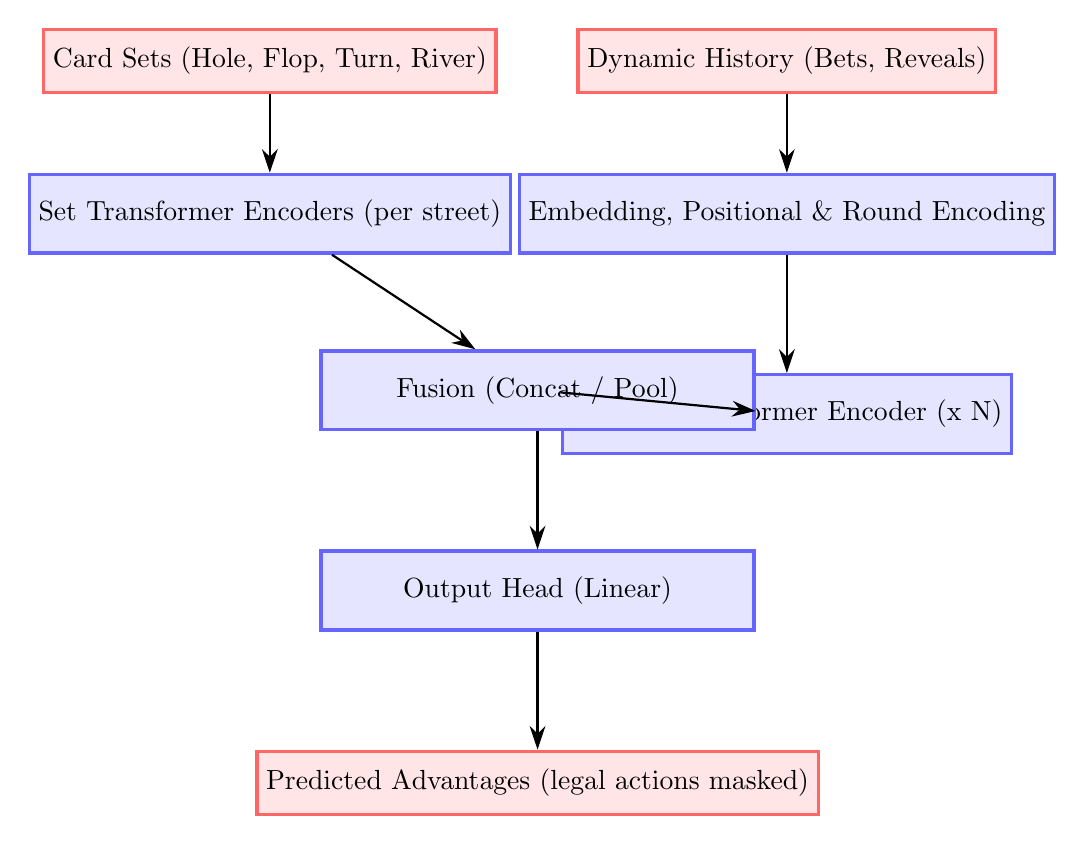
\begin{tikzpicture}[
    node distance=1.5cm,
    block/.style={rectangle, draw=blue!60, fill=blue!10, very thick, minimum height=1cm, minimum width=5.5cm},
    input/.style={rectangle, draw=red!60, fill=red!10, very thick, minimum height=0.8cm, minimum width=4.2cm},
    arrow/.style={-{Stealth[length=3mm, width=2mm]}, thick}
]

% Nodes
\node (CardSets) [input] {Card Sets (Hole, Flop, Turn, River)};
\node (HistSeq) [input, right=1cm of CardSets] {Dynamic History (Bets, Reveals)};

\node (SetEnc) [block, below=1cm of CardSets] {Set Transformer Encoders (per street)};
\node (EmbedHist) [block, below=1cm of HistSeq] {Embedding, Positional \& Round Encoding};

\node (HistTransformer) [block, below=of EmbedHist] {History Transformer Encoder (x N)};

\node (Fusion) [block, below=1.2cm of SetEnc, xshift=3.4cm] {Fusion (Concat / Pool)};
\node (OutputHead) [block, below=of Fusion] {Output Head (Linear)};

\node (Output) [input, below=of OutputHead] {Predicted Advantages (legal actions masked)};

% Arrows
\draw [arrow] (CardSets) -- (SetEnc);
\draw [arrow] (HistSeq) -- (EmbedHist);
\draw [arrow] (EmbedHist) -- (HistTransformer);
\draw [arrow] (SetEnc) -- (Fusion);
\draw [arrow] (HistTransformer) -- (Fusion);
\draw [arrow] (OutputHead) -- (Output);
\draw [arrow] (Fusion) -- (OutputHead);

\end{tikzpicture}
\caption{Proposed all-Transformer architecture: permutation-invariant card-set encoders fused with a Transformer history encoder to produce advantages over legal abstract actions.}
\label{fig:architecture}
\end{figure}

\section{Implementation Details and Challenges}

\subsection{Action Abstraction and Translation}

While Deep CFR reduces the need for \textit{information abstraction}, \textit{action abstraction} is required in NLHE due to the continuous space of bet sizes. Implementations restrict legal bets to a discrete set per street (e.g., \{0.5x, 1x, 2x pot, all-in\}) with standard min-raise rules.

Crucially, when deployed, an \textbf{action translation} mechanism is required. If an opponent makes an off-tree bet size, the system maps it back into the abstraction (e.g., to the nearest sizes). To reduce bias and discontinuities, we optionally use \emph{stochastic interpolation} between the two nearest sizes. When available, a stronger alternative is \textbf{nested subgame re-solving} (safe re-solving) that starts a small search at the off-tree node using the blueprint as a prior.

While action abstraction is a practical necessity for CFR-based methods, it is worth noting that alternative deep reinforcement learning frameworks have explored outputting a continuous probability distribution over bet sizes. Such approaches, often based on policy gradient methods, face their own challenges in imperfect-information games, including high variance and difficulty in converging to a Nash equilibrium, which is why the discrete action space approach combined with robust translation remains the dominant paradigm in state-of-the-art poker AI.

\subsection{Efficient Distributed Infrastructure}

Training requires a distributed Actor-Learner architecture.
\begin{enumerate}
    \item \textbf{Actors (Data Generators):} Parallel CPU processes execute the MCCFR traversals (External Sampling). They utilize the latest $V_A$ weights and push data into centralized, concurrent Memory Buffers.
    \item \textbf{Learners (Trainers):} GPU/TPU workers continuously sample batches from the Memory Buffers (respecting the LCFR weighting as per the normalized loss) to update the Transformer weights. Following Deep CFR, we periodically \emph{retrain from scratch} on the buffer to reduce drift and overfitting to recent samples.
\end{enumerate}
The efficiency of the game logic and traversal code (often implemented in C++ or Rust) is frequently the system bottleneck.

\subsection{Computational Scale and Requirements}

A project of this magnitude requires significant computational resources, comparable to large language model training.
\begin{itemize}
    \item \textbf{Model and Memory:} The Transformer model itself might consist of 6-12 encoder layers with a model dimension of 512-1024, resulting in 50-200 million parameters. The main memory buffer ($M_A$) for reservoir sampling typically needs to hold $10^8$ to $10^9$ training samples (infoset, regret, iteration tuples).
    \item \textbf{Compute Resources:} The distributed setup relies on heterogeneous hardware. The \textbf{Actors} are CPU-bound and require thousands of parallel cores to generate data efficiently; the performance of the underlying game engine (typically C++ or Rust) is critical. The \textbf{Learner} requires one or more high-end accelerators (e.g., NVIDIA A100/H100 GPUs or a Google TPU Pod slice) for training the network.
    \item \textbf{Training Duration:} A full training run from scratch can consume several days to weeks, accumulating thousands of GPU-hours for the learner and tens of thousands of CPU-hours for the actors.
\end{itemize}

\subsection{Avoiding Common CFR Errors}

Rigorous validation of the CFR logic is essential, especially when basing implementation on existing codebases which may contain subtle errors.

\begin{itemize}
    \item \textbf{Incorrect Reach Probabilities:} This is the most critical error. CFVs \textit{must} be weighted by the opponent's reach probability ($\pi_{-i}$) \emph{and chance}. Using the player's own reach probability ($\pi_{i}$) breaks the definition of the Counterfactual Value and the theoretical guarantees of CFR.
    \item \textbf{Improper Sampling in MCCFR:} External Sampling must correctly sample chance and opponent actions according to the \textit{current} strategy profile $\sigma^T$. Biased sampling leads to incorrect regret estimates.
    \item \textbf{Errors in Weighted Loss Calculation:} As detailed above, LCFR weighting must be applied using the iteration index of each sample, with \emph{normalized} weighted MSE to stabilize gradients.
    \item \textbf{Information Leakage:} Ensure the infoset representation strictly adheres to the definition and does not include hidden information.
    \item \textbf{Training Stability and Initialization:} Transformers require careful learning rate scheduling (e.g., warm-up and decay with AdamW) and gradient clipping. Periodically retraining from scratch on the full buffer helps avoid drift.
    \item \textbf{Legal-Action Masking:} The advantage head must be masked to legal actions prior to regret-matching; if all advantages are non-positive, fall back to uniform over legal actions.
    \item \textbf{Context: CFR+}: Regret-matching+ (CFR+) speeds up tabular CFR; with function approximation it is less direct, but worth noting for context \cite{tammelin2014cfrplus}.
\end{itemize}

Validation should always begin by testing the framework on smaller games (e.g., Kuhn or Leduc poker) and verifying that exploitability converges towards zero.

\section{Evaluation}

Evaluating a poker AI involves assessing how closely it approximates a Nash equilibrium and how robustly it plays under off-tree perturbations.

\begin{enumerate}
    \item \textbf{Exploitability (e):} The theoretical measure of performance; exact computation is intractable for NLHE.
    \item \textbf{Approximate Best Response (ABR):} Estimate exploitability with Local Best Response (LBR) or related ABR procedures against the reconstructed average strategy.
    \item \textbf{Performance Benchmarking:} Evaluate on HU NLHE (e.g., 100bb) against strong baselines (tabular/abstraction CFR, Deep CFR with MLP head, NFSP) and report win rate in milli-big blinds per game (mbb/g) with confidence intervals over large samples.
    \item \textbf{Ablations:} (i) Transformer vs. MLP advantage networks; (ii) card-set encoder on/off; (iii) LCFR on/off; (iv) retrain-from-scratch vs. continuous fine-tuning; (v) action translation: deterministic nearest vs. stochastic interpolation vs. optional nested re-solving.
\end{enumerate}

\section{Conclusion}

Deep CFR provides a powerful framework for tackling the complexity of HU NLHE by generalizing strategic knowledge through function approximation. Using \emph{only} Transformer components—permutation-invariant card-set encoders fused with a history encoder—aligns naturally with poker's structure. Successful implementation requires careful CFR accounting (reach probabilities and sampling), normalized LCFR weighting, robust handling of off-tree actions, and disciplined evaluation against standard baselines.

\bibliographystyle{plain}
% References
\begin{thebibliography}{99}

\bibitem{brown2017superhuman}
Noam Brown and Tuomas Sandholm.
\newblock Superhuman AI for heads-up no-limit poker: Libratus beats top professionals.
\newblock {\em Science}, 356(6337):508--513, 2017.

\bibitem{brown2019superhuman}
Noam Brown and Tuomas Sandholm.
\newblock Superhuman AI for multiplayer poker.
\newblock {\em Science}, 365(6456):885--890, 2019.

\bibitem{brown2018deep}
Noam Brown, Adam Lerer, Sam Gross, and Tuomas Sandholm.
\newblock Deep counterfactual regret minimization.
\newblock In {\em International Conference on Machine Learning (ICML)}, pages 793--802. PMLR, 2019. (First appeared as arXiv preprint arXiv:1811.00164, 2018).

\bibitem{vaswani2017attention}
Ashish Vaswani, et al.
\newblock Attention is all you need.
\newblock In {\em Advances in neural information processing systems (NeurIPS)}, 2017.

\bibitem{zinkevich2007regret}
Martin Zinkevich, et al.
\newblock Regret minimization in games with incomplete information.
\newblock In {\em Advances in neural information processing systems (NeurIPS)}, 2007.

\bibitem{moravcik2017deepstack}
Matej Moravcik, Martin Schmid, Neil Burch, Viliam Lisý, Dustin Morrill, Nolan Bard, Trevor Davis, Kevin Waugh, Michael Johanson, and Michael Bowling.
\newblock DeepStack: Expert-level artificial intelligence in heads-up no-limit poker.
\newblock {\em Science}, 356(6337):508--513, 2017.

\bibitem{brown2020rebel}
Noam Brown, Anton Bakhtin, Adam Lerer, and Qianggong Zhang.
\newblock ReBeL: A general framework for self-play in imperfect-information games.
\newblock {\em arXiv preprint arXiv:2007.13544}, 2020.

\bibitem{steinberger2019sdcfr}
Eric Steinberger.
\newblock Single Deep CFR: One neural network to approximate them all.
\newblock {\em arXiv preprint arXiv:1901.07621}, 2019.

\bibitem{lee2019settransformer}
Juho Lee, Yoonho Lee, Jungtaek Kim, Adam Kosiorek, Seungjin Choi, and Yee Whye Teh.
\newblock Set Transformer: A framework for attention-based permutation-invariant neural networks.
\newblock In {\em ICML}, 2019.

\bibitem{tammelin2014cfrplus}
Oskari Tammelin.
\newblock Solving large imperfect information games using CFR+.
\newblock In {\em AAAI Workshop on Computer Poker and Imperfect Information Games}, 2014.

\bibitem{lanctot2009mccfr}
Marc Lanctot, Kevin Waugh, Martin Zinkevich, and Michael Bowling.
\newblock Monte Carlo sampling for regret minimization in extensive games.
\newblock In {\em NIPS}, 2009.

\bibitem{schmid2018vrmccfr}
Martin Schmid, Neil Burch, Matej Moravcik, and Michael Bowling.
\newblock Variance reduction in Monte Carlo counterfactual regret minimization (VR-MCCFR).
\newblock In {\em AAMAS}, 2018.

\bibitem{heinrich2016nfsp}
Johannes Heinrich and David Silver.
\newblock Deep reinforcement learning from self-play in imperfect-information games (Neural Fictitious Self-Play).
\newblock {\em arXiv preprint arXiv:1603.01121}, 2016.

\bibitem{johanson2013sizing}
Michael Johanson.
\newblock Measuring the size of large no-limit poker games.
\newblock {\em Technical Report}, 2013.

\end{thebibliography}

\end{document}